\documentclass{standalone}
\usepackage{tikz}
\usetikzlibrary{patterns, positioning}
\usetikzlibrary{shapes.misc}
\usepackage[outline]{contour}
\contourlength{1.5pt} 
\usepackage[sfdefault]{ClearSans} %% option 'sfdefault' activates Clear Sans as the default text font
\usepackage[T1]{fontenc}

\begin{document}
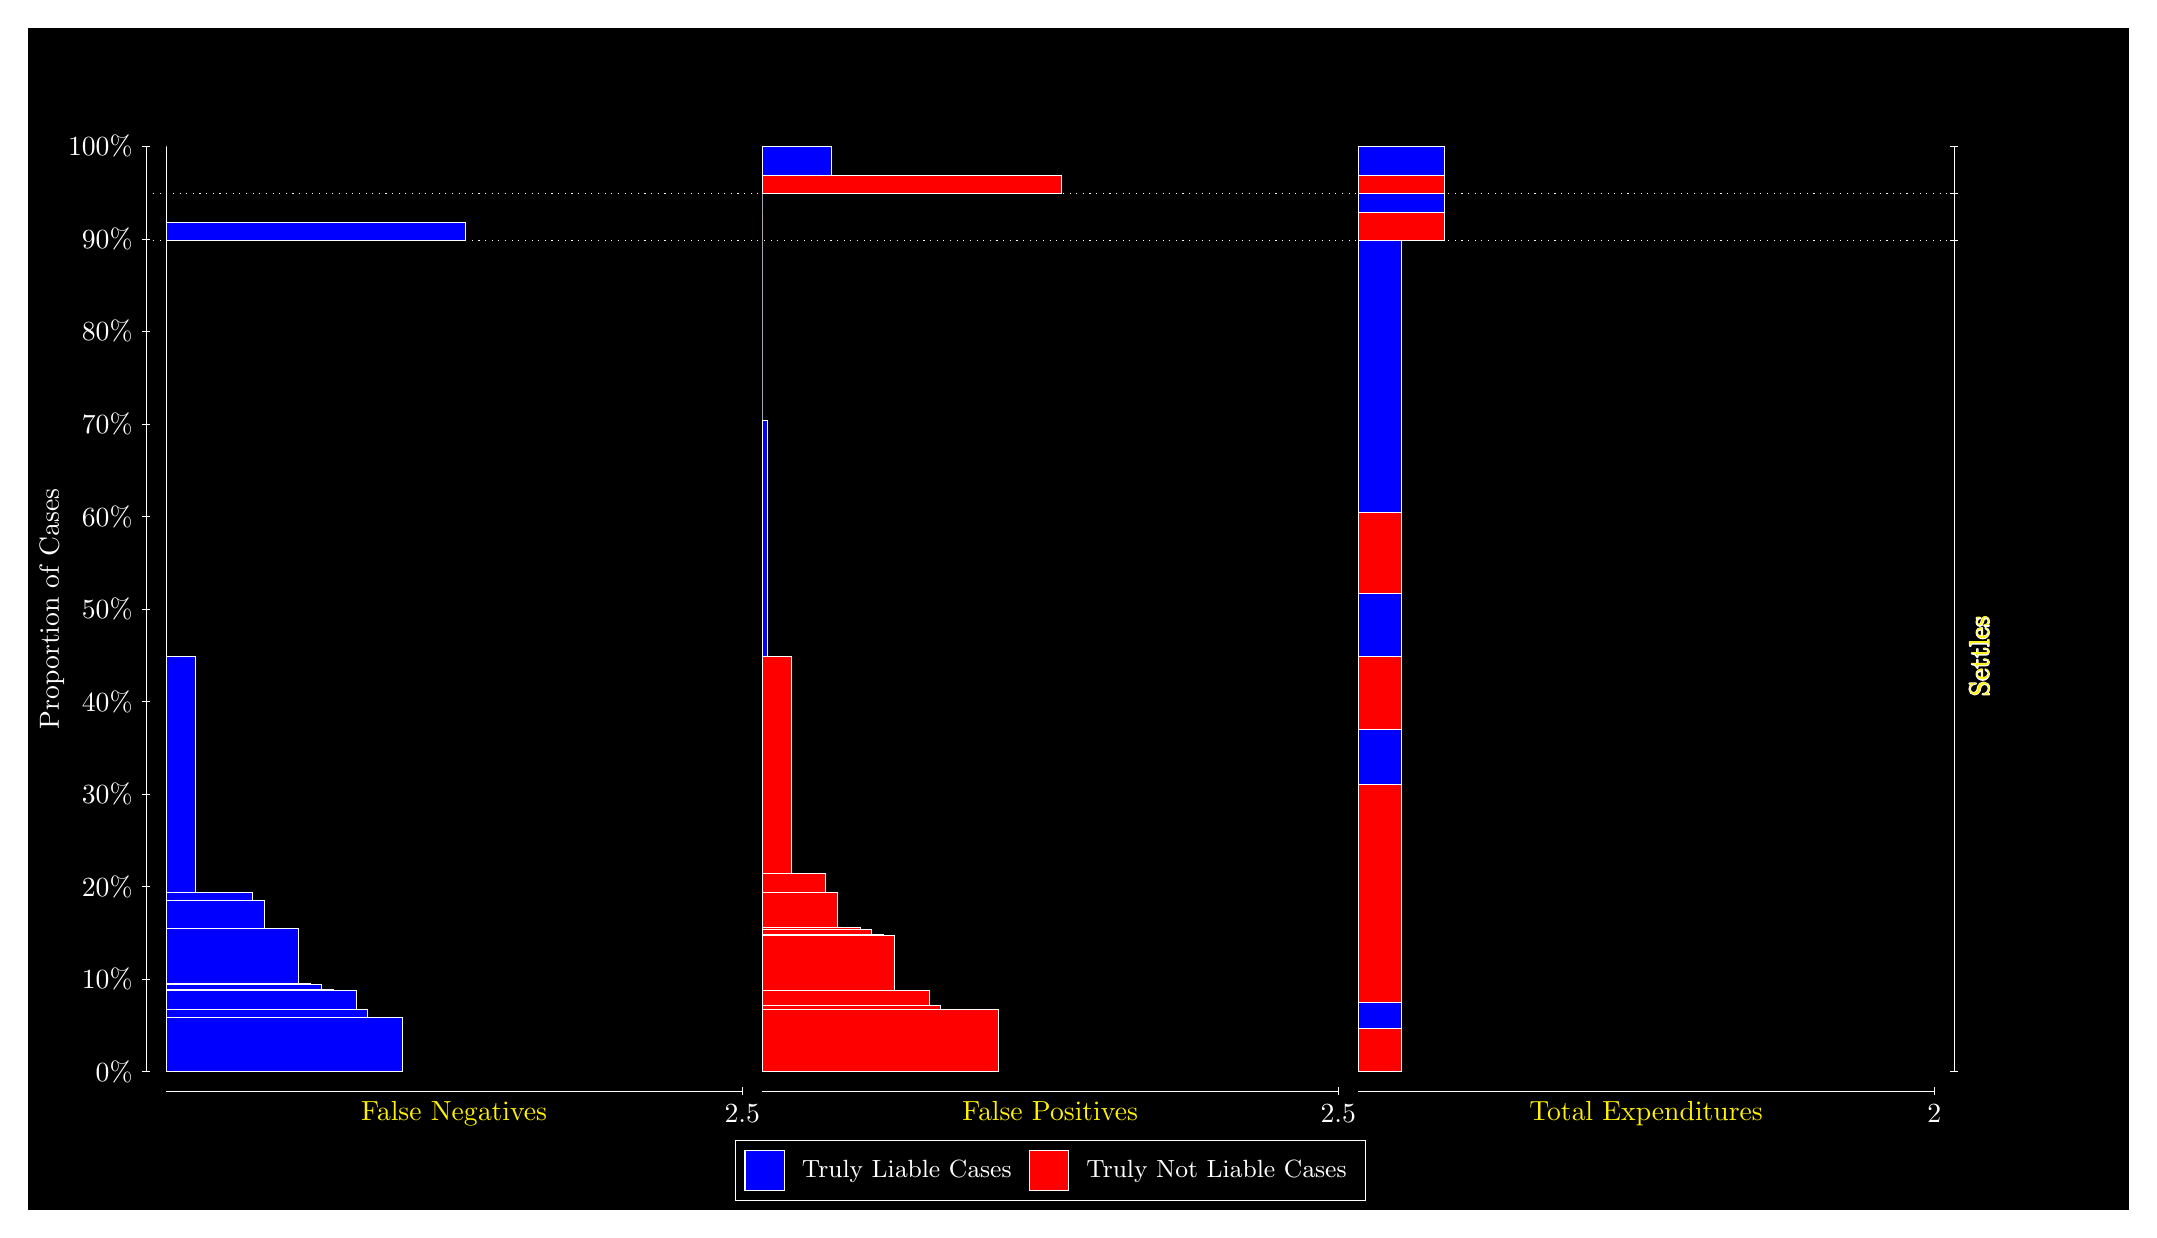
\begin{tikzpicture}
\draw[fill=black] (0,0) rectangle (26.667,15);
\draw[white, very thin] (1.5,1.75) -- (1.5,13.5);
\node[rotate=90, text=white, anchor=center] at (0.3, 7.625) {Proportion of Cases};
\draw[white, very thin] (1.45,1.75) -- (1.55,1.75);
\node[text=white, anchor=east] at (1.45, 1.75) {0\%};
\draw[white, very thin] (1.45,2.925) -- (1.55,2.925);
\node[text=white, anchor=east] at (1.45, 2.925) {10\%};
\draw[white, very thin] (1.45,4.1) -- (1.55,4.1);
\node[text=white, anchor=east] at (1.45, 4.1) {20\%};
\draw[white, very thin] (1.45,5.275) -- (1.55,5.275);
\node[text=white, anchor=east] at (1.45, 5.275) {30\%};
\draw[white, very thin] (1.45,6.45) -- (1.55,6.45);
\node[text=white, anchor=east] at (1.45, 6.45) {40\%};
\draw[white, very thin] (1.45,7.625) -- (1.55,7.625);
\node[text=white, anchor=east] at (1.45, 7.625) {50\%};
\draw[white, very thin] (1.45,8.8) -- (1.55,8.8);
\node[text=white, anchor=east] at (1.45, 8.8) {60\%};
\draw[white, very thin] (1.45,9.975) -- (1.55,9.975);
\node[text=white, anchor=east] at (1.45, 9.975) {70\%};
\draw[white, very thin] (1.45,11.15) -- (1.55,11.15);
\node[text=white, anchor=east] at (1.45, 11.15) {80\%};
\draw[white, very thin] (1.45,12.325) -- (1.55,12.325);
\node[text=white, anchor=east] at (1.45, 12.325) {90\%};
\draw[white, very thin] (1.45,13.5) -- (1.55,13.5);
\node[text=white, anchor=east] at (1.45, 13.5) {100\%};

\draw[white, very thin] (24.457,1.75) -- (24.457,13.5);
\draw[white, very thin] (24.407,1.75) -- (24.507,1.75);
\node[anchor=west] at (24.407, 1.75) {};
\draw[white, very thin] (24.407,12.302) -- (24.507,12.302);
\node[anchor=west] at (24.407, 12.302) {};
\draw[white, very thin] (24.407,12.898) -- (24.507,12.898);
\node[anchor=west] at (24.407, 12.898) {};
\draw[white, very thin] (24.407,13.5) -- (24.507,13.5);
\node[anchor=west] at (24.407, 13.5) {};

\draw[white, very thin, fill=blue] (1.75,1.75) rectangle (4.7507,2.4451);
\draw[white, very thin, fill=blue] (1.75,2.4451) rectangle (4.3116,2.5418);
\draw[white, very thin, fill=blue] (1.75,2.5418) rectangle (4.1652,2.7799);
\draw[white, very thin, fill=blue] (1.75,2.7799) rectangle (3.8725,2.7987);
\draw[white, very thin, fill=blue] (1.75,2.7987) rectangle (3.7261,2.8585);
\draw[white, very thin, fill=blue] (1.75,2.8585) rectangle (3.5797,2.8762);
\draw[white, very thin, fill=blue] (1.75,2.8762) rectangle (3.4333,3.5738);
\draw[white, very thin, fill=blue] (1.75,3.5738) rectangle (2.9942,3.9244);
\draw[white, very thin, fill=blue] (1.75,3.9244) rectangle (2.8478,4.0279);
\draw[white, very thin, fill=blue] (1.75,4.0279) rectangle (2.1159,7.0236);
\draw[white, very thin, fill=red] (1.75,7.0236) rectangle (1.75,12.302);
\draw[white, very thin, fill=blue] (1.75,12.302) rectangle (5.5558,12.537);
\draw[white, very thin, fill=red] (1.75,12.537) rectangle (1.75,12.898);
\draw[white, very thin, fill=red] (1.75,12.898) rectangle (1.75,13.134);
\draw[white, very thin, fill=blue] (1.75,13.134) rectangle (1.75,13.5);
\draw[white, very thin, fill=red] (9.3189,1.75) rectangle (12.32,2.5383);
\draw[white, very thin, fill=red] (9.3189,2.5383) rectangle (11.588,2.5934);
\draw[white, very thin, fill=red] (9.3189,2.5934) rectangle (11.441,2.7799);
\draw[white, very thin, fill=red] (9.3189,2.7799) rectangle (11.002,3.4775);
\draw[white, very thin, fill=red] (9.3189,3.4775) rectangle (10.856,3.4951);
\draw[white, very thin, fill=red] (9.3189,3.4951) rectangle (10.709,3.5549);
\draw[white, very thin, fill=red] (9.3189,3.5549) rectangle (10.563,3.5779);
\draw[white, very thin, fill=red] (9.3189,3.5779) rectangle (10.27,4.0255);
\draw[white, very thin, fill=red] (9.3189,4.0255) rectangle (10.124,4.2632);
\draw[white, very thin, fill=red] (9.3189,4.2632) rectangle (9.6848,7.0279);
\draw[white, very thin, fill=blue] (9.3189,7.0279) rectangle (9.3921,10.024);
\draw[white, very thin, fill=blue] (9.3189,10.024) rectangle (9.3189,12.302);
\draw[white, very thin, fill=red] (9.3189,12.302) rectangle (9.3189,12.662);
\draw[white, very thin, fill=blue] (9.3189,12.662) rectangle (9.3189,12.898);
\draw[white, very thin, fill=red] (9.3189,12.898) rectangle (13.125,13.134);
\draw[white, very thin, fill=blue] (9.3189,13.134) rectangle (10.197,13.5);
\draw[white, very thin, fill=red] (16.888,1.75) rectangle (17.437,2.298);
\draw[white, very thin, fill=blue] (16.888,2.298) rectangle (17.437,2.6324);
\draw[white, very thin, fill=red] (16.888,2.6324) rectangle (17.437,5.3971);
\draw[white, very thin, fill=blue] (16.888,5.3971) rectangle (17.437,6.0922);
\draw[white, very thin, fill=red] (16.888,6.0922) rectangle (17.437,7.0275);
\draw[white, very thin, fill=blue] (16.888,7.0275) rectangle (17.437,7.8218);
\draw[white, very thin, fill=red] (16.888,7.8218) rectangle (17.437,8.8517);
\draw[white, very thin, fill=blue] (16.888,8.8517) rectangle (17.437,12.302);
\draw[white, very thin, fill=red] (16.888,12.302) rectangle (17.986,12.662);
\draw[white, very thin, fill=blue] (16.888,12.662) rectangle (17.986,12.898);
\draw[white, very thin, fill=red] (16.888,12.898) rectangle (17.986,13.134);
\draw[white, very thin, fill=blue] (16.888,13.134) rectangle (17.986,13.5);
\draw[white, dotted] (1.5,12.302) -- (24.457,12.302);
\draw[white, dotted] (1.5,12.898) -- (24.457,12.898);
\draw[white, very thin] (1.75,1.5) -- (9.0689,1.5);
\node[text=yellow, anchor=north] at (5.4094, 1.5) {False Negatives};
\draw[white, very thin] (9.0689,1.45) -- (9.0689,1.55);
\node[text=white, anchor=north] at (9.0689, 1.45) {2.5};

\draw[white, very thin] (9.3189,1.5) -- (16.638,1.5);
\node[text=yellow, anchor=north] at (12.978, 1.5) {False Positives};
\draw[white, very thin] (16.638,1.45) -- (16.638,1.55);
\node[text=white, anchor=north] at (16.638, 1.45) {2.5};

\draw[white, very thin] (16.888,1.5) -- (24.207,1.5);
\node[text=yellow, anchor=north] at (20.547, 1.5) {Total Expenditures};
\draw[white, very thin] (24.207,1.45) -- (24.207,1.55);
\node[text=white, anchor=north] at (24.207, 1.45) {2};

\node[text=yellow, centered, rotate=90] at (24.777, 7.0258) {\contour{white}{Settles}};



\draw (12.978300999999998,1.5) node[draw=none] (baseCoordinate) {};
\begin{scope}[align=center]
        \matrix[scale=0.5, draw=white, below=0.5cm of baseCoordinate, nodes={draw}, column sep=0.1cm]{
            \node[rectangle, draw, minimum width=0.5cm, minimum height=0.5cm, fill=blue] {}; &
            \node[draw=none, font=\small, text=white] (B) {Truly Liable Cases}; &
            \node[rectangle, draw, minimum width=0.5cm, minimum height=0.5cm, fill=red] {}; &
            \node[draw=none, font=\small, text=white] (B) {Truly Not Liable Cases}; \\
            };
\end{scope}

\end{tikzpicture}
\end{document}